\cotefile{43}
\scanpage{32}
% archive sheet number: 31
% s1, lines 1--3
{\unsure{Utilisant}} une technique de descente analogue, on \deleted{{\unsure{et}}} définit {\unsure{par descente}} un homomorphisme
\[
H^1(X,G)\xrightarrow{d}\operatorname{Hom}_{Y\text{-}\mathrm{grp}}(G_m,G)
\qquad (\uline{\text{{\unsure{hom degré|hom. de gr.}}}})
\]
% margin note slanted; two-ended reference line points to the preceding display
\margin{{\unsure{la définition dans le cas général à voir au cas}} $Y=\operatorname{Spec}(k)$, $k$ {\unsure{alg. clos}}, $G=G_m$ {\unsure{\ldots}}}
\diagram{\begin{tikzcd}[ampersand replacement=\&]{}\arrow[r,leftrightarrow]\&{}\end{tikzcd}}
et on trouve que {\unsure{la suite}}
\[
\boxed{0\longrightarrow \operatorname{Ext}^1({\unsure{\mathscr{P}|\Phi}}_{X/{\unsure{Y|k}}},G)
\longrightarrow H^1({\unsure{X_S|X,S|X}},G)
\longrightarrow\operatorname{Hom}_{Y\text{-}\mathrm{grp}}(G_m,G)}
\]
est exacte. {\unsure{Il est même plausible que}} cette suite s'insère dans la suite exacte prolongée
\[
\boxed{\longrightarrow\operatorname{Ext}^2(\mathscr{P}_{X/Y},G)
\longrightarrow H^2(X,G)\longrightarrow\operatorname{Ext}^1_{Y\text{-}\mathrm{grp}}(G_m,G)\longrightarrow\cdots}
\]
où {\unsure{on fera paraître|a faire paraître}} l'hom
\[
\operatorname{Ext}^i(G_m,G)\longrightarrow\operatorname{Ext}^{i+2}(\mathscr{P}_{X/Y},G)
\]
est la multiplication par un élément fondamental
\[
{\unsure{\zeta|\xi}}\in\operatorname{Ext}^2_{Y\text{-}\mathrm{grp}}(\mathscr{P}_{X/Y},G_m)
\]
dont la définition {\unsure{directe}}; la formule {\unsure{serait}} la suivante [{\unsure{valable}} s'il existe un $S$ {\unsure{étale}} tq $S\to Y$ soit surjectif,
\scanpage{33}
% archive sheet number: 32
condition toujours remplie lorsque $S$ est local :

On considère l'extension
\[
0\longrightarrow N_S\longrightarrow{\unsure{\mathscr{P}|\Phi}}_{S{\unsure{,}}X/Y}\longrightarrow\mathscr{P}_{X/Y}\longrightarrow 0
\]
d'où un
\[
\xi\in\operatorname{Ext}^1(\mathscr{P}_{X/Y},N_S)
\]
puis l'extension
\[
0\longrightarrow G_{m{\unsure{,}}Y}\longrightarrow\deleted{{\unsure{G}}}{\unsure{\mathscr{S}|\mathscr{I}}}_{X/Y/S}\longrightarrow N_S\longrightarrow 0
\]
d'où un
\[
\eta\in\operatorname{Ext}^1(N_S,G_{m,Y})
\]
et on pose
\[
\zeta=\eta\circ\xi
\]
\uline{Dans le cas où} ${\unsure{\deleted{\zeta}\xi|\xi}}=0$, \uline{par exemple s'il existe une section de} $X$ sur ${\unsure{Y}}$ ({\unsure{qui|que}} {\unsure{l'on peut en définir alors}} $\zeta$, {\unsure{qui sera nulle car alors on aura}} $\eta=0$] on aura donc les suites exactes {\unsure{triviales}} suivantes
\[
\boxed{0\longrightarrow\operatorname{Ext}^i(\mathscr{P}_{X/Y},G)\longrightarrow H^i(X,G)\longrightarrow\operatorname{Ext}^{i-1}(G_m,G)\longrightarrow0}
\]
\scanpage{34}
% archive sheet number: 33
% Left-hand page of the open sheet.
\figure{\begin{tikzpicture}\draw (0,0)--(1.2,0);\draw (0.05,.13)--(1.3,.13);\end{tikzpicture}}
Passant à la limite sur des $S$ de plus en plus {\unsure{grands|petits}} (et {\unsure{faisceautisant}} sur $Y$, pour pouvoir le faire) on trouve un \inserted{pro $Y$-}schéma en {\unsure{grps}} ${\unsure{\mathscr{P}|\Phi}}_{\infty\,X/Y}$, \deleted{{\unsure{fini}}} et un \deleted{{\unsure{pro-morphisme}}}\inserted{{\unsure{pro-application}}} rationnelle {\unsure{transverse}} aux fibres de $X/Y$
\[
{\unsure{\varphi|\phi}}_\infty:X\longrightarrow\mathscr{P}_\infty^1
\]
qui sera solution d'un problème universel relatif aux {\unsure{pro-morphismes}} {\unsure{transverses}} aux fibres de $X/Y$ dans les fibrés principaux sous des $Y$-schémas en groupes \inserted{\uline{commutatifs}} de type fini. On aura alors, si ${\unsure{\mathscr{R}|R}}_{X/Y}\deleted{{\unsure{X}}}$ désigne la \uline{{\unsure{cat. fibrée}}} sur $Y$ définie par $X$
\[
\deleted{{\unsure{\underline{H}^1(\mathscr{R})}}}
\left\{\begin{aligned}
\operatorname{Hom}_{{\unsure{Y}}}({\unsure{\mathscr{R}_{X/Y}^1|\mathscr{R}_{X/Y}}},P^1)&\xleftarrow{\sim}\operatorname{Hom}_{Y\text{-}\mathrm{grp}}(\mathscr{P}_\infty^1,P)\\
\underline{H}^0(\mathscr{R}_{X/Y},G)&\xleftarrow{\sim}\deleted{{\unsure{\operatorname{Ext}^0}}}{\unsure{\underline{\operatorname{Hom}}}}_{Y\text{-}\mathrm{grp}}(\mathscr{P}_\infty,G)\\
\underline{H}^1(\mathscr{R}_{X/Y},G)&\xleftarrow{\sim}\operatorname{Ext}^1_{Y\text{-}\mathrm{grp}}(\mathscr{P}_\infty,G)\\
&\text{et sans doute}\\
\underline{H}^i(\mathscr{R}_{X/Y},G)&\xleftarrow{\sim}\operatorname{Ext}^i_{Y\text{-}\mathrm{grp}}(\mathscr{P}_\infty,G)
\end{aligned}\right.
\]
% margin note slanted, beside the brace of the last displays
\margin{{\unsure{isom de|D'où}} faisceaux sur $S$}

\figure{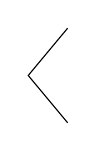
\begin{tikzpicture}\draw (0,1)--(-.5,.4)--(0,-.2);\end{tikzpicture}}
% Right-hand page.
{\unsure{Je voudrais|Je note}} : {\unsure{lier}} les $\operatorname{Ext}^i(\mathscr{P}_{S,X/S},G)$ avec les $\operatorname{Ext}^{{\unsure{i|0}}}(\mathscr{P}^0_{S,X/S},G)$ que l'on considère d'habitude. Le lien se fait par la suite exacte des $\operatorname{Ext}$ {\unsure{déduite}} de
\[
0\longrightarrow\mathscr{P}_S^0\longrightarrow\mathscr{P}_S\longrightarrow\mathbb{Z}\longrightarrow0\tag*{(*)}
\]
donnant donc
\diagram{\begin{tikzcd}[ampersand replacement=\&,column sep=small,row sep=small]
\&\&\operatorname{Hom}(X-S,G)\arrow[d,phantom,"{\tikz[baseline=-.5ex]{\node[rotate=90] {$\simeq$};}}"]\&\&\& H^1(X-S,G)\arrow[d,phantom,"{\tikz[baseline=-.5ex]{\node[rotate=90] {$\simeq$};}}\,?"]\\
0\arrow[r]\&H^0(S,G)\arrow[r]\&\operatorname{Hom}(\mathscr{P}_S,G)\arrow[r]\&\operatorname{Hom}(\mathscr{P}_S^0,G)\arrow[r]\&H^1(S,G)\arrow[r]\&\operatorname{Ext}^1(\mathscr{P}_S,G)
\end{tikzcd}}
\diagram{\begin{tikzcd}[ampersand replacement=\&,column sep=small,row sep=small]
\&\&\&H^2(X-S,G)\arrow[d,phantom,"{\tikz[baseline=-.5ex]{\node[rotate=90] {$\simeq$};}}\,?"]\\
{}\arrow[r]\&\operatorname{Ext}^1(\mathscr{P}_S^0,G)\arrow[r]\&H^2(S,G)\arrow[r]\&\operatorname{Ext}^2(\mathscr{P}_S,G)\arrow[r]\&\cdots
\end{tikzcd}}
\figure{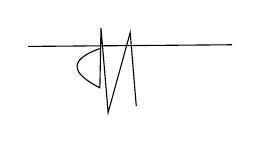
\begin{tikzpicture}[scale=.7]
\draw (0,1.1)--(3.7,1.13);\draw (1.3,1.06)..controls (.7,.85) and (.8,.6)..(1.3,.35)--(1.32,1.43)--(1.45,-.1)--(1.85,1.35)--(1.96,.02);
\end{tikzpicture}}
On notera que dans cette théorie, [du moins pour les {\unsure{courbes}}] on n'a aucun besoin de notion de symbole local, encore moins de la théorie des Jacobiennes locales, qui en un sens semble plus subtile {\unsure{------}}
\scanpage{35}
% archive sheet number: 34
{\unsure{Difficulté|Difficile}}

\diagram{\begin{tikzcd}[ampersand replacement=\&,column sep=large,row sep=large]
0\arrow[r]\&\underset{\substack{\text{faisceau de}\\\text{Picard relatif}\\\text{\uline{{\unsure{réduit}}} (?)}}}{\underline{{\unsure{\mathscr{P}|\Phi}}}(X/Y)_0}\arrow[r]\&\underline{\operatorname{Ext}}^1(\mathscr{P}^0_{X/Y},G_m)\arrow[d,"{\unsure{2|\sim}}","\substack{\text{\uline{autodualité de}}\\\text{\uline{la Jacobienne}}}"']\\
\&\&\deleted{{\unsure{\mathscr{P}^0}}}\underline{H}^0(Y,\mathscr{P}^0_{X/Y})
\end{tikzcd}}
\figure{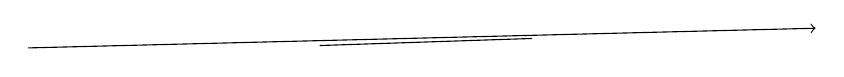
\begin{tikzpicture}\draw[->] (0,0)--(10,.25);\draw (3.7,.03)--(6.4,.12);\end{tikzpicture}}
\margin{sur ${\unsure{Y}}$}
La réciproque semble {\unsure{vraie}} pour les faisceaux de {\unsure{Weil}}. Ceci dit, on doit avoir sous des conditions convenables
\diagram{\begin{tikzcd}[ampersand replacement=\&,column sep=large,row sep=small]
\underline{\underline{H}}^*(X_S/{\unsure{Y}},G)\&\underline{\underline{\operatorname{Ext}}}^*(\mathscr{P}_S,G)\arrow[l,"\sim"']\arrow[d,"2"]\\
\&\underline{\underline{\operatorname{Ext}}}^{{\unsure{2|*|\geq}}}(\mathscr{P}_S^0,G)\quad\text{en }\underline{\underline{\text{dim }>0}}
\end{tikzcd}}
D'autre part, on a \deleted{{\unsure{une}}} \inserted{des} suites spectrales,
\[
\begin{aligned}
\operatorname{Ext}^*(\mathscr{P}_S,G)&\Longleftarrow H^p(Y,\underline{\underline{\operatorname{Ext}}}^{q}(\mathscr{P}_S,G))\\
\underset{\deleted{\underline{\phantom{H}}}}{H}^*(X_S/Y,G)&\Longleftarrow H^p({\unsure{Y}},\underline{\underline{H}}^q(X_S/Y,G))
\end{aligned}
\]
d'où en \deleted{substituant une suite spectrale}
\[
\deleted{\boxed{H^*(X_S/Y,G)\Longleftarrow H^p(Y,\underline{\underline{\operatorname{Ext}}}^{q}(\mathscr{P}_S,G))}}
\]
\deleted{d'où une suite exacte à 5 termes}

{\unsure{comprenant}} le résultat plausible
\[
{\unsure{H}}^*(X_S/Y,G)\simeq\operatorname{Ext}_S^*(\mathscr{P}_S,G)
\]
\margin{$\deleted{0\longrightarrow H^1(Y,\underline{\operatorname{Hom}}(\mathscr{P}_S,G))}$}
\scanpage{36}
% archive sheet number: 35
Adèles des {\unsure{proschémas}}
\scanpage{37}
% archive sheet number: 36
${\unsure{\mathscr{S}|S}}_\infty$ schéma d'anneaux \inserted{{\unsure{affine}}} sur $\mathbb{Z}$, si $A$ est un anneau, on a
\[
\mathscr{S}_\infty({\unsure{\mathbb{Z}|A}})=A[[t]]^{**}
\]
(séries formelles d'augmentation 1) où l'addition est la multiplication des séries formelles, et le produit est la convolution $*$. Il y a aussi des opérations $\lambda^i$. {\unsure{Rappelons}},
\[
(1+at)*f(t)=f(at)\qquad\text{i.e. }\{1+at\}\{f(t)\}=\{f(at)\}
\]
% margin note written sideways
\margin{{\unsure{Relations}} {\unsure{séries|liens|bien}} {\unsure{formelles}} et {\unsure{vecteurs de Witt}}}
Si $A$ est de car $p>0$, on aura un \uline{endomorphisme} $F$ de $\mathscr{S}_\infty(A)$ [provenant de l'endomorphisme de Frobenius de $\mathscr{S}_{\infty\,\mathbb{Z}/p\mathbb{Z}}$]
\[
F\left(\sum a_it^i\right)=\sum a_i^pt^i
\]
\figure{\begin{tikzpicture}\fill(0,0)circle(.015);\fill(.15,-.02)circle(.015);\draw(.25,.03)--(.4,.07);\draw(.48,-.12)--(.59,-.08);\fill(-.05,-.2)circle(.01);\end{tikzpicture}}
et on aura
\[
\deleted{{\unsure{F(f(at))}}}\quad f(t)^p=F(f)(t^p)
\]
Cela conduit alors à poser
\[
V(f)(t)=f(t^p)
\]
[$V$ est un {\unsure{endomorphisme|monomorphisme}} additif] et on aura
\[
FV(\{f\})=VF(\{f\})=p\{f\}.
\]
N.B. $F$ est aussi un endomorphisme pour la structure d'anneaux

En \deleted{{\unsure{a donc}}} par exemple
\[
(1+xt^{p^i})*f(t)=F^i(f)(xt^{p^i})
\]
car \deleted{{\unsure{si $x=a^{p^i}$, le premier membre est}} {\unsure{donc le membre}} ${\unsure{1+ax}}$}
\[
\begin{aligned}
(1+at)^{p^i}*f&=f(at)^{p^i}\\
&=F^i(f)(a^{p^i}t^{p^i})=F^i(f)(xt^{p^i}).
\end{aligned}
\]
Sans restriction \deleted{\illegible{1}} de caractéristique, on a un morphisme d'anneaux
\[
\psi:\mathscr{S}_\infty\longrightarrow W_\infty^{{\unsure{p}}}\qquad[\text{anneau de Witt pour le nb premier }p]
\]
\margin{?}
qui en tant que morphisme additif est déterminé par
\[
\psi(\{1+at\})=\epsilon(a)=(a,0,0,\ldots)
\]
\scanpage{38}
% archive sheet number: 37
(cela {\unsure{marche parce que}} l'application $\epsilon$ : ``{\unsure{représentant}} multiplicatif est {\unsure{fonctorielle}}, i.e. provient d'un morphisme de $\mathbb{Z}$-schémas $G_a\longrightarrow W_\infty$).
\scanpage{40}
% archive sheet number: 39
\[
0\longrightarrow K^*\longrightarrow\prod_{\mathrm{local}}K_x^*\longrightarrow{\unsure{\mathbb{J}|\mathscr{J}}}_C(\bar{k})\longrightarrow0
\]
% margin note slanted, circled
\margin{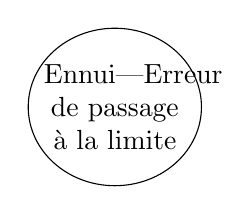
\begin{tikzpicture}\node[text width=1.8cm,align=center] (n) {\uline{{\unsure{Ennui|Erreur}} de passage à la limite}};\draw (n.center) ellipse (1.1cm and 1cm);\end{tikzpicture}}
\margin{\textcircled{?}}
\[
\begin{aligned}
\widehat H^*(\Gamma,K^*)&=0&&\text{par le théorème de Tsen global}\\
\widehat H^*(\Gamma,K_x^*)&=0&&\text{''}\qquad\text{local}
\end{aligned}
\]
d'où
\[
\widehat H^*(\Gamma,\mathbb{J}_C(\bar{k}))=0\qquad\text{géométrique}
\]
\[-\]
En particulier

\deleted{${\unsure{H}}\ C^*(\Gamma,\mathbb{J}_C({\unsure{k|\bar{k}}}))$ est une \uline{résolution} de ${\unsure{\mathbb{J}}}$. \inserted{$H^0(C^*(\Gamma,\mathbb{J}_C({\unsure{\bar{k}}})))$}}

$C^*(\Gamma,\mathbb{J}_C(\bar{k}))$ est une \uline{résolution} de $H^0(\Gamma,\mathbb{J}_C(\bar{k}))$

Or on a, en vertu de $H^1(\Gamma,K^*)=0$
\[
\begin{aligned}
H^0(\Gamma,\mathbb{J}_C(\bar{k}))&=H^0\left(\prod_{\substack{\mathrm{local}\\x\in X}}K_x^*\right)/\operatorname{Im}H^0(K^*)\\
&=\left(\prod_{\substack{\mathrm{local}\\x'\in X'}}K_{x'}^{\prime *}\right)/K^{\prime *}=\mathbb{J}_{C'}(\bar{k})
\end{aligned}
\]
C'est là une résolution \inserted{(Mais qui {\unsure{ne sont pas|ne soit pas|n'est pas}} ``{\unsure{admissibles|admissible}}'')} de \uline{$\pi$-groupes}

D'où
\[
H^*(\pi,\mathbb{J}_{C'}(\bar{k}))\Longleftarrow H^p\left(H^q\left(\pi,\underbrace{C^*\left(\Gamma,\mathbb{J}_C(\bar{k})\right)}_{C^*(\Gamma,\mathbb{J}_C)(\bar{k})}\right)\right)
\]
\[
\begin{aligned}
q>0\qquad H^q(\pi,C^*(\Gamma,\mathbb{J}_C)(\bar{k}))
&=\deleted{{\unsure{C^*}}}H^q(\pi,C^*(\Gamma,\mathbb{Z}))=0\\[-2pt]
&\qquad\text{(Lang)}
\end{aligned}
\]
\margin{trivial car $C^*(\Gamma,\mathbb{Z})$ est $\simeq\mathbb{Z}^{{\unsure{(I)|I}}}$ \deleted{{\unsure{\mathbb{Z}}}}}
\[
q=0\qquad C^*(\Gamma,\mathbb{J}_C(\bar{k}))^\pi=C^*(\Gamma,\mathbb{J}_C(k))
\]
\figure{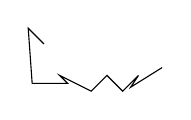
\begin{tikzpicture}\draw (0,.5)--(-.2,.7)--(-.15,0)--(.3,0)--(.2,.1)--(.6,-.1)--(.8,.1)--(1,-.1)--(1.2,.1)--(1.1,-.05)--(1.5,.2);\end{tikzpicture}}
\scanpage{41}
% archive sheet number: 40
% The manuscript is upside down in the supplied scan; transcription follows it after a 180-degree rotation.
\[
H^p(k,\underline{\underline{H}}^q(\Gamma,{\unsure{\mathbb{J}|\mathscr{J}}}_{C'}))
\quad\deleted{{\unsure{=\ \underline{\underline{H}}^p\ H^p}}}\qquad H^p(k,\mathbb{J}_C)\qquad\deleted{{\unsure{\Gamma|\mathbb{J}}}}\mathbb{J}_C(k)
\]
\[
H^p(H^q(k,\underline{\underline{C}}^*(\Gamma,\mathbb{J}_{C'}))
\]
\[
\overset{q=0}{H^p(C^*(\Gamma,\mathbb{J}_{C'}))}=H^p(\Gamma,\mathbb{J}_{C'})
\]
\diagram{\begin{tikzcd}[ampersand replacement=\&,column sep=large,row sep=small]
\mathbb{J}_{C'}(\bar{k})\&\underline{C}(\underbrace{\Gamma^n,\mathbb{J}_{C'}})(\bar{k})\&\text{\uline{résolution} de }\mathbb{J}_C(\bar{k})\\
\Gamma\quad\pi\&{}\arrow[u]\&\text{par des }\pi\text{-}{\unsure{\mathrm{grps}}}
\end{tikzcd}}
\[
H^*(\pi,\mathbb{J}_C(\bar{k}))\Longleftarrow H^p(H^q(\pi,\underline{C}(\Gamma^{{\unsure{\bullet|n}}},\mathbb{J}_{C'})(\bar{k})))
\]
\[
\begin{array}{cc}
{\tikz[baseline=-.5ex]{\node[rotate=90] {$=$};}}&\\
\mathbb{J}_C(k)&H^q(\pi,\underline{C}(\Gamma^{\bullet},\mathbb{Z}))\quad\substack{q>0\\=0}
\end{array}
\]
\[
H^0(\Gamma,\mathbb{J}_{C'}(\bar{k}))\qquad\deleted{{\unsure{H^0\in}}}C(\Gamma^{\bullet},\mathbb{J}_{C'})
\]
\[
\hfill{\unsure{H^p|H_p}}(\Gamma,\mathbb{J}_{C'}(k))
\]
\[
\deleted{H}\qquad 1\qquad\underset{\deleted{{\unsure{=}}}}{C}
\]
\[
\Gamma\qquad C(\Gamma^n,\mathbb{J}_{C'}^{{\unsure{\bullet|0}}})
\]
\[
\mathbb{J}_C(\bar{k})\longrightarrow\underline{\mathbb{J}_{C'}(\bar{k})}\longrightarrow\mathbb{J}_{C'}(\bar{k})^\Gamma\longrightarrow\mathbb{J}_{C'}(\bar{k})^{\Gamma^2}
\]
\diagram{\begin{tikzcd}[ampersand replacement=\&,row sep=small,column sep=small]
(\delta{\unsure{\varphi|\phi}})(x)\&{}=\varphi({\unsure{\sigma|\gamma}}x)-\varphi(x)\\
\Gamma\arrow[u]\&\tau_\sigma\varphi-\varphi
\end{tikzcd}}
\scanpage{42}
% archive sheet number: 41
\[
\deleted{C^*(\Gamma}\quad\varprojlim\underbrace{H^*\left(\pi,{\unsure{\mathbb{J}|\mathscr{J}}}_{C',\alpha}(\bar{k})\right)}_{\begin{aligned}
&=H^i(\pi,\mathbb{Z})=0\quad\text{si }i>0\\
&=H^0(\pi,\mathbb{J}_{C',\alpha}(\bar{k}))=\mathbb{J}_{C',\alpha}(k)\quad\text{satisfait M.L.}
\end{aligned}}=\mathbb{J}_{C'}(k)
\]
\[
H^p\bigl(\varprojlim_\alpha\underbrace{H^q(\pi,C^*(\Gamma,\mathbb{J}_{C,\alpha}(\bar{k}))}_{\begin{aligned}
\deleted{q>0}\quad&=H^q(\pi,C^*(\Gamma,{\unsure{\mathbb{Z}}}))=0\qquad\text{si }q>0\\
&=\underbrace{H^0(\pi,C^*(\Gamma,\mathbb{J}_{C,\alpha}(\bar{k})))=C^*(\Gamma,\mathbb{J}_{C,\alpha}(k))}_{\underbrace{C^*(\Gamma,\mathbb{J}_C(k))}}
\end{aligned}}
\]
\diagram{\begin{tikzcd}[ampersand replacement=\&,column sep=small,row sep=large]
\deleted{{\unsure{N|\mathbb{J}}}}\,\alpha E^1\arrow[r]\&G\&{}\arrow[d]\&{}\\
\operatorname{Ext}^1({\unsure{J}}^0/N,G)\&\&H^2(k,G)\arrow[d]\&H^p(\Gamma,\mathbb{J}_C(k))\\
H^1(K,G)\&\&\operatorname{Ext}^1(J_K,G)\arrow[ll,"\sim"']\arrow[d]\&\widehat{\mathbb{Z}}\arrow[r]\&0\\
G\quad C^i(G)\&\&\operatorname{Ext}^1(J_K^0,G)\arrow[d]\&{}\\
H^p({\unsure{\mathscr{H}|H}}\&\&H^2(k,G)=0\&{}
\end{tikzcd}}
\diagram{\begin{tikzcd}[ampersand replacement=\&,column sep=large,row sep=small]
0\arrow[r]\&H^0({\unsure{k}},\Gamma)\arrow[r]\&\operatorname{Hom}(J_K,\Gamma)\arrow[r,dash]\&\operatorname{Hom}(J_K^0,\Gamma)\\
\&\Gamma\arrow[u,phantom,"{\tikz[baseline=-.5ex]{\node[rotate=90] {$=$};}}"]\&\Gamma\&{}
\end{tikzcd}}
\figure{
\begin{tikzpicture}
\draw[line width=1.6pt] (-.35,-.4)--(.35,.4);\draw[line width=1.6pt](-.42,0)--(.42,0);\draw[line width=1.6pt](-.2,.43)--(.2,-.43);
\draw (1.1,-.35)--(1.6,.35);\draw (1,-.1)--(1.75,.1);\draw (1.15,.4)--(1.65,-.4);
\node[anchor=west] at (3,0) {$\operatorname{Ext}^1(J^0,\Gamma)=\operatorname{Hom}$};
\draw[->] (7.4,.5)--(3,.5)--(2.7,-.45);
\end{tikzpicture}}
\scanpage{43}
% archive sheet number: 42
\[
\operatorname{Ext}^{1}\bigl(J,\underset{\substack{\downarrow\\\text{{\unsure{grp fini}}}}}{G}\bigr)\Rightarrow\operatorname{Hom}.(J(k),G(k))
\]
\[ - \]
\diagram{\begin{tikzcd}[ampersand replacement=\&,column sep=large]
J(k)\&{}\times\operatorname{Ext}^{1}(J,G) \arrow[r] \& \boxed{H^1(k,G)\simeq G(k)} \\
H^0(k,J) \arrow[u,equal] \&\& \text{(corps fini)} \\
\operatorname{Hom}(\mathbb Z,J) \&\& \operatorname{Hom}(J(k),G(k))
\end{tikzcd}}
\diagram{\begin{tikzpicture}
\node[anchor=west] at (0,0) {\begin{tikzcd}[ampersand replacement=\&,column sep=small,row sep=small]
0\arrow[r]\&G\arrow[r]\&E\arrow[r]\&J\arrow[r]\&{\unsure{0|\cdot}}\\
\&\&\&\mathbb Z\arrow[u]\&
\end{tikzcd}};
\draw (2.7,-1) -- (5.5,-1) .. controls (6.2,-.9) and (6.1,1.5) .. (6.6,1.9) -- (11.5,2.1);
\draw (2.7,-1.1) -- (5.5,-1.02);
\draw (6.6,1.75) -- (11.6,1.98);
\draw (6.6,1.75) -- (6.75,1.69) -- (6.69,1.61);
\node at (7.1,.8) {${\unsure{J^1|J'}}$};
\end{tikzpicture}}
\[\pi_1(J)-\pi_1(\mathbb Z)\]
\diagram{\begin{tikzcd}[ampersand replacement=\&,column sep=small,row sep=large]
0\arrow[r]\&\operatorname{Ext}^1(\mathbb Z,G)\arrow[r]\arrow[d,"{\unsure{2|\sim}}"']\&\operatorname{Ext}^1({\unsure{\mathbb J|J}},G)\arrow[r]\arrow[d]\&\operatorname{Ext}^1(\mathbb J^0 G)\arrow[r]\arrow[d,"2"]\&0\\
0\arrow[r]\&\operatorname{Hom}(\mathbb Z,H^1(G))\arrow[r]\&\operatorname{Hom}(\mathbb J(k),H^1(G))\arrow[r]\&\operatorname{Hom}(\mathbb J^0(k),H^1(G))\arrow[r,dash]\&0
\end{tikzcd}}
\scanpage{45}
% archive sheet number: 44
\[\prod_{x\in X}\widehat{{\unsure{\mathscr O|\mathcal O}}}_x\]
\margin{{\unsure{Adèles}} pour plusieurs {\unsure{dimensions}}}
\figure{\begin{tikzpicture}\draw (0,1.5) .. controls (.1,1) and (-.1,.3) .. (0,0) -- (4,0);\end{tikzpicture}}
\[\prod_{\substack{\mathrm{local}\\x_1\in X_1}}\widehat{\mathscr O}_{x_1}\otimes_{\underline{\mathscr O}_{x_1}}K=\prod_{\mathrm{local}}K_D\]
\[\prod_{x_1}\deleted{{\unsure{\mathrm{lim}|\mathrm{loc}}}}\prod_{\substack{\mathrm{local}\\\underline{x_0}\in\bar x_1}}\mathscr O_{[x_0,x_1]}\]
\diagram{\begin{tikzcd}[ampersand replacement=\&,column sep=large]
\displaystyle\prod_{x_0x_1(x_2)}\mathscr O_{[x_0x_1x_2]}\arrow[d]\&\mathscr O_{[x_0x_2]}=\widehat{\underline{\mathscr O}}_{x_0}\otimes_{\underline{\mathscr O}_{x_0}}K\\
\mathscr O_{[x_0x_1]}\otimes_{\mathscr O_{x_1}}K\&
\end{tikzcd}}
\diagram{\begin{tikzcd}[ampersand replacement=\&,column sep=tiny,row sep=large]
K\arrow[d,equal]\&\underbrace{\longrightarrow}_{\widehat{\mathscr O}_{x_1}\otimes_{\underline{\mathscr O}_{x_1}}K}\&I_{x_1}\&\underbrace{\longrightarrow}_{\underline{\mathscr O}_{[x_0,x_1]}}\&I_{x_0}\\
\widehat{\underline{\mathscr O}}_{x_2}\&\&\widehat{\deleted{{\unsure{t|b}}}\underline{\mathscr O}}_{{\unsure{x_p|x_1}}}\&\&\widehat{\underline{\mathscr O}}_{x_0}
\end{tikzcd}}
\figure{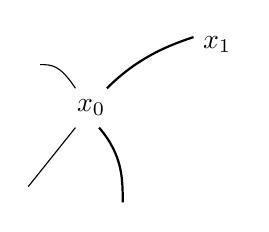
\begin{tikzpicture}
\node at (0,0) {$x_0$};\node at (1.6,.8) {$x_1$};
\draw[thick] (.2,.25) .. controls (.6,.65) and (1,.8) .. (1.3,.9);
\draw (-.2,.25) .. controls (-.4,.55) and (-.5,.55) .. (-.65,.55);
\draw (-.2,-.25) -- (-.8,-1);
\draw[thick] (.1,-.25) .. controls (.4,-.6) and (.4,-.9) .. (.4,-1.2);
\end{tikzpicture}}
\[\begin{array}{ccc}\widehat{\underline{\mathscr O}}_{x_0}&\widehat{\mathscr O}_{x_1}&\widehat{\mathscr O}_{x_2}\\{\unsure{m_0|\mathfrak m_0}}&m_1&m_2\end{array}\]
\[\prod_{x\in X}\mathscr O_{[x]}\]
\[\prod_{\substack{\mathrm{local}\\x_1\in X_1}}\mathscr O_{[x_1,x_2]}\qquad{\unsure{\mathscr O.}}\]
\[\prod_{x_1}\prod_{\substack{\mathrm{local}\\x_0}}\mathscr O_{[x_0,x_1]}\]
\figure{\begin{tikzpicture}\draw (0,0)--(.5,1.8);\end{tikzpicture}}
\diagram{\begin{tikzcd}[ampersand replacement=\&,column sep=small,row sep=large]
\displaystyle\prod_{\underline{x_0}}\mathscr O_{[x_0]}\arrow[d,"\text{{\unsure{localisat|localisant}}}"]\&\&\\
\displaystyle\prod_{\underline{x_1}}\prod_{\substack{\mathrm{local}\\\underline{x_0}}}\mathscr O_{[x_0,x_1]}\arrow[d,"\overline{\text{{\unsure{localisat|localisant}}}}"]\&\displaystyle\prod_{\underline{x_1}}\mathscr O_{[\bar x_1]}\arrow[l]\arrow[d,"\text{{\unsure{localisant|localisat}}}"]\&\\
\displaystyle\prod_{\substack{{\unsure{\mathrm{rest.}|\mathrm{restr.}}}\\\underline{x_0}}}\prod_{\substack{\mathrm{rest.}\\\underline{x_1}}}\mathscr O_{[x_0,x_1,x_2]}\&\displaystyle\prod_{\substack{\mathrm{local}\\(\underline{\underline{x_1}},x_2)}}\mathscr O_{[\bar x_1x_2]}\arrow[l]\&\displaystyle\prod_{x_2}\mathscr O_{[x_2]}=K\arrow[l]
\end{tikzcd}}
\[\underline{\mathscr O}_{[\underline{\underline{x_1}},x_2]}\qquad\deleted{\prod_{x_1}}\]
\[\deleted{{\unsure{\mathscr A|\mathcal A}}_{i_0--i_{p-1}}}\qquad\deleted{{\unsure{\sum x_1|\prod}}_{x_1}}\]
\figure{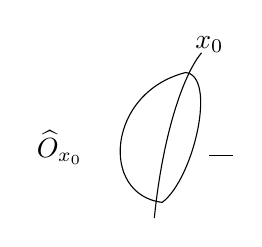
\begin{tikzpicture}
\node at (-1.3,-.3) {$\widehat{\mathscr O}_{x_0}$};\node at (.6,1) {$x_0$};
\draw (0,-1) .. controls (-.8,-.9) and (-.7,.4) .. (.3,.65) .. controls (.7,.6) and (.4,-.7) .. (0,-1);
\draw (-.1,-1.2) .. controls (0,-.2) and (.25,.6) .. (.5,.9);
\draw (.6,-.4)--(.9,-.4);
\end{tikzpicture}}
\diagram{\begin{tikzcd}[ampersand replacement=\&,row sep=small]
\mathscr O_{[x_0x_1]}\arrow[d]\\
\displaystyle\prod_{x_0x_1}\mathscr O_{[x_0x_1x_2]}
\end{tikzcd}}
\[\mathscr A_{i_0--i_p}\qquad\mathscr A_{i_1\cdots i_{p-1}}\]
\deleted{{\unsure{localisé|localis.}}}
\[x_{i_0}\quad x_{i_1}-x_{i_p}\]
\[i_0<i_1<\cdots<i_p\]
\[-\]
\scanpage{46}
% archive sheet number: 45
\[{\unsure{\mathscr A|\mathcal A}}^{*}=\prod_{x\in X}\mathscr A^{*}_{{\unsure{\pi_x|\Pi_x}}}\]
\[\mathscr A^{*}_{\pi_x}=\varprojlim_{{\unsure{n|u}}}(\mathscr A^{*}_{\pi_x})/\]
\scanpage{47}
% archive sheet number: 46
\[\varprojlim_i{\unsure{\mathscr A|\mathcal A}}^{0}\otimes_A\mathscr A^0/{\unsure{\mathfrak m_i|\mathfrak n_i|\pi_i}}\qquad\prod\widehat{{\unsure{\underline{\mathscr O}|\underline{\mathcal O}}}}_x\otimes_A K\]
\[\mathscr A^0\otimes_A\mathscr A^0/\mathfrak m_i\subset\prod_{x\in X}\widehat{\underline{\mathscr O}}_x\otimes_A\mathscr O_a/{\unsure{m_a^n|\mathfrak m_a^n}}=\prod_{\substack{\deleted{{\unsure{x\in X|x\leq a}}}\\x\leq a}}\widehat{\mathscr O}_x\otimes\mathscr O_a/m_a^n\]
\[\prod_a\varprojlim_n\bigl(\prod_{x\leq a}\widehat{\mathscr O}_x\otimes\mathscr O_a/m_a^n\bigr)\]
\[\text{''}\]
\[\deleted{a\in X_{{\unsure{i|1}}}}\qquad\prod_a\varprojlim_{{\unsure{n|-}}}\bigl[(\widehat{\mathscr O}_a\otimes\mathscr O_a/m_a^n)\times(\prod_{x<a}\widehat{\mathscr O}_x)\otimes\mathscr O_a/m_a^n)\bigr]\]
\[\text{''}\]
\[\prod_a\widehat{\mathscr O}_a\times\prod_i\underbrace{\prod_{{\unsure{a\in X_i|a^i\in X_i}}}\varprojlim_n\bigl((\prod_{x<a}\widehat{\mathscr O}_x)\otimes\underline{\mathscr O}_a/m_a^n\bigr)}_{\begin{array}{ll}i=0&0\\i=1&(\prod_{x<a}\widehat{\mathscr O}_x)\otimes\mathscr O_a/m_a^n\\i=2&(\prod_{x<a}\widehat{\mathscr O}_x)\otimes K\end{array}}\]
\figure{\begin{tikzpicture}
\node at (0,1) {$\deleted{{\unsure{a_i=0}}}$};
\node at (-.4,-.1) {$\deleted{{\unsure{a_i}}}$};
\node at (.5,.4) {$\deleted{{\unsure{\mathscr A^i=}}}$};
\draw (-.1,.95)--(-.3,0)--(1.4,.1);\draw (-.4,.85)--(1.5,.9);
\draw (.2,.1)--(.8,.9)--(.8,.2)--(1.3,.8);
\draw (1.3,.6)..controls(1.6,.3)and(1.8,.9)..(2.3,1.1);
\draw (2.1,1) ellipse (.09,.05);\draw (2.3,1.1) ellipse (.08,.04);
\end{tikzpicture}}
\[\begin{aligned}
\mathscr A^n&=\deleted{{\unsure{\mathscr A}}}\varprojlim_\alpha\mathscr A^{n-1}\otimes_A\mathscr A^0/\mathfrak m_\alpha\\
&=\prod_{a\in X}\varprojlim_k\mathscr A^{{\unsure{n-2|n-1}}}\otimes_A\mathscr O_a/m_a^k
\end{aligned}\]
\diagram{\begin{tikzcd}[ampersand replacement=\&,row sep=small]
{}\arrow[d,phantom,"\cap" description]\\
\displaystyle\prod_{x_0\leq x_1\leq\cdots\leq x_n}\mathscr A_{[x_0,\ldots,x_n]}
\end{tikzcd}}
\margin{\uline{{\unsure{l'inclusion étant|l'immersion étant}}} \uline{{\unsure{fidèlement}} {\unsure{plate}}}}
% slanted
\[\mathscr A^{n+1}=\prod_{a\in X}\varprojlim_k\mathscr A^n\otimes_A\mathscr O_a/m_a^k\subset\prod_{a\in X}\varprojlim_{{\unsure{u|n}}}\underbrace{(\prod_{x_0\leq\cdots\leq x_n}\mathscr A_{[x_0--x_n]})\otimes\mathscr O_a/m_a^{{\unsure{k|u}}}}_{\displaystyle\subset\prod_{x_0\leq\cdots\leq x_n}\mathscr A_{[x_0--x_n]}{\unsure{\otimes\mathscr O_a/}}}\]
\[\mathscr A_{[x_0,\ldots x_n,a]}\qquad{\unsure{1|\prime}}\qquad\text{''}\]
\scanpage{48}
% archive sheet number: 47
\figure{\begin{tikzpicture}\draw (0,1.4)..controls(1,.9)and(1.5,.1)..(1.5,-.8);\draw (.8,.7) ellipse (.25,.35);\draw[rotate around={-35:(1,.3)}] (1,.3) ellipse (.35,.23);\fill (.8,.7) circle (.05);\end{tikzpicture}}
\[\prod\widehat{{\unsure{\underline{\mathscr O}|\underline{\mathcal O}}}}_x\otimes_{\mathscr O_x}K\]
\[\widehat{\mathscr O}_x\otimes_{\underline{\mathscr O}_x}\deleted{{\unsure{K_x|L_x}}}L_{{\unsure{n|u}}}\]
\figure{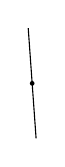
\begin{tikzpicture}\draw (0,-.7)--(-.1,.7);\fill (-.05,0) circle (.03);\end{tikzpicture}}
\diagram{\begin{tikzcd}[ampersand replacement=\&,column sep=small,row sep=large]
\widehat{\mathscr O}_x\otimes_{\mathscr O_x}({\unsure{m|\mathfrak m}}^n/m^{{\unsure{n+1|n}}})_{{\unsure{v|\nu}}}\arrow[r]\&\widehat{\mathscr O}_x\otimes L_{{\unsure{n+1|u n}}}\arrow[r,dash]\&\widehat{\underline{\mathscr O}}_x\otimes L_n\\
\&\widehat{\mathscr O}_{\deleted{{\unsure{x}}}}/m^{n+1}\arrow[u,"*\quad *"]\arrow[r]\&\widehat{\mathscr O}_{\deleted{x}}/m^n\arrow[u,"*"]\\
\&*\&*
\end{tikzcd}}
\diagram{\begin{tikzcd}[ampersand replacement=\&,row sep=small]
k[[s,t]]\&\\
k[s,t]\arrow[u]\arrow[r]\&k[s,t]_{(s)}\\
m\&
\end{tikzcd}}
\[\deleted{{\unsure{K|t}}}\qquad\begin{array}{ccc}x_0&x_0&x_0\\x_1&x_1&\deleted{{\unsure{x_1|x}}}\\x_{{\unsure{1|2}}}&x_{{\unsure{1|2}}}&x_1\\&x&x_2\end{array}\]
\margin{$\prod\widehat{\underline{\mathscr O}}_x$}
% margin note written sideways
\margin{$(\widehat{\underline{\mathscr O}}_x^{\deleted{*}}\otimes_{\mathscr O_x}K)^*$}
% margin note written sideways
\diagram{\begin{tikzcd}[ampersand replacement=\&,row sep=large]
k[s]\\
\begin{array}{c}x_0\\x_2\end{array}\arrow[u]
\end{tikzcd}}
\[\widehat{\mathscr O}_{{\unsure{x|2}}}\deleted{{\unsure{\otimes_{\mathscr O_x}}}}{\unsure{\varpi|\pi|\mathfrak p}}\mathscr O_v/\varpi\mathscr O_v-\widehat{\mathscr O}_x\otimes_{\mathscr O_v}\varpi\mathscr O_v/\varpi^{{\unsure{2}}}\mathscr O_v-\widehat{\mathscr O}_x\otimes_{\mathscr O_v}L\]
\diagram{\begin{tikzcd}[ampersand replacement=\&,row sep=small]
{\unsure{\mathscr A|\mathcal A}}_{i_0--i_{p-1}}\arrow[d]\&\\
\mathscr A_{i_0---i_p}.\&\mathscr A_{i_p}\arrow[l]
\end{tikzcd}}
\[\widehat{\mathscr O}_{{\unsure{u|x}}}\longrightarrow\widehat{\mathscr O}_x\ S^{-1}\]
\[\varpi\qquad\varpi^2\]
\figure{\begin{tikzpicture}\draw[thick] (0,0) ellipse (.45,.35);\draw(-.1,-.34)..controls(.1,0)and(0,.2)..(-.1,.34);\draw(-.6,.2)..controls(-.3,0)and(.3,-.2)..(.43,-.05);\end{tikzpicture}}
\[k[[t]][\deleted{{\unsure{s}}}s]/(s^{{\unsure{n}}}\]
\margin{$k[[s,t]]$}
% margin note written sideways
\[\mathscr A_{[p_0,--p_n]}\otimes_A A_{p_{n+1}},{\unsure{p_{n-1}|p_{n+1}}},A_{p_n}\]
\margin{-- {\unsure{localiser}} en les {\unsure{polynômes}} en $s,t$ qui {\unsure{ne sont pas}} {\unsure{multiples}} de $s$}
\[a_0(t)+a_1(t)s{\unsure{\sim|\cdots}}+a_{n-1}(t)s^{n-1}\]
\[a_0(t)[1+a_0(t)^{-1}a_1(t)s\sim\]
\[A_{[p_0]}\widehat\otimes_A\underline{A_{[p_1]}}\]
\[\widehat{\mathscr O}_x\otimes K\]
\diagram{\begin{tikzcd}[ampersand replacement=\&,row sep=large]
\deleted{a_0}\quad k((t))[s]/(s^n)\\
k[[s,t]]\arrow[u]
\end{tikzcd}}
\[\mathscr A_{\ell_0,\ell_1,\ldots,\ell_p}\qquad\mathscr A_{\ell_{p+1}}\qquad\mathscr A_{{\unsure{\ell|2}}}\]
\figure{\begin{tikzpicture}\draw (0,1.2)..controls(.8,.4)and(1,-.2)..(1.15,-1);\draw(.65,-.35)..controls(1,-.1)and(1.3,-.05)..(1.4,-.12);\node at (1.15,-1.25) {$s=0$};\end{tikzpicture}}
\[\underline{\underline{a_0(t)}}+\underline{\underline{a_1(t)}}s\sim+\underline{\underline{a_{n-1}(t)}}s^{n-1}\]
\[\mathscr A_1\qquad\mathscr A_{[{\unsure{X|x}}]}^{\otimes}\]
\[\mathscr O_x\quad\mathscr A_0\quad\otimes.\]
\[\varprojlim\widehat A\otimes_A A/{\unsure{\mathfrak m_i|\mathfrak n_i|\pi_i}}\]
\[\varprojlim A\]
\[\begin{aligned}k((t))[[s]]\\k[[t]][[s]]\\k((t))/k[[t]]\qquad[[s]]\end{aligned}\]
